\documentclass[11pt,a4paper]{article}

\usepackage[utf8]{inputenc}
\usepackage[english]{babel}
\usepackage[T1]{fontenc}

\usepackage{amsmath,amssymb,amsfonts}

\usepackage{tikz}
\usetikzlibrary{shapes,arrows}
\usepackage{tkz-graph}

\usepackage{graphicx}
\usepackage{hyperref}

\title{Advanced Algorithms\\Assignment 1}
\author{Kristoffer Søholm \ \ \ Sebastian Paaske Tørholm \ \ \  Oskar Behrendt}

\begin{document}
\maketitle

\section{Exercise 1: $b$-flow}
We can express a $b$-flow problem as a max-flow problem. Let every vertex,
v, with positive demand get an edge from the source with capacity $b_v$, and
every vertex $v$ with negative demand get an edge to the sink with capacity
$-b_v$. If we in this network can get a maximum flow that maxes out all of both
the source and sink edges, we have a corresponding $b$-flow.
This, however, was not what we were asked about.

Figure $1(a)$ does have a $b$-flow, as can be seen in \autoref{fig-a-bflow}.

Figure $1(b)$ does not have one, since no flow can leave $v_4$, and thus it
cannot satisfy the requirement of $b_4 = -2$.

\begin{figure}[h!]
    \centering
    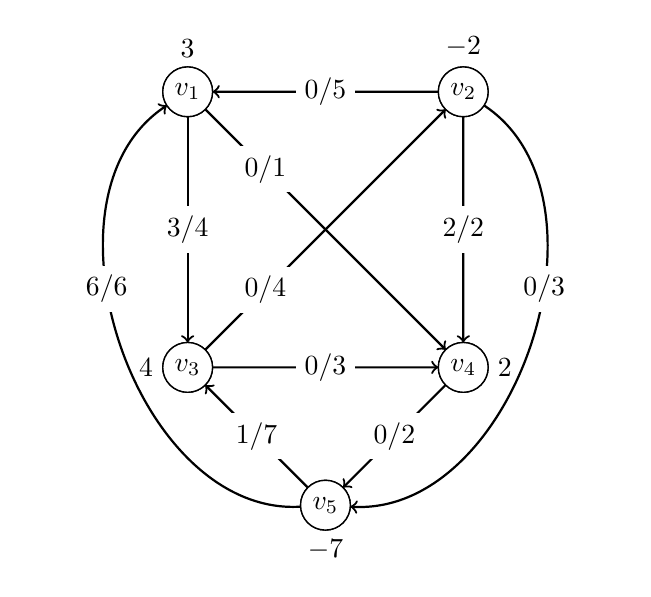
\begin{tikzpicture}[scale=1.75]
        \tikzset{EdgeStyle/.style={->}}

        \Vertex[x=0,y=3,L= 3,Math=true,LabelOut,Lpos=90]{D1}
        \Vertex[x=2,y=3,L=-2,Math=true,LabelOut,Lpos=90]{D2}
        \Vertex[x=0,y=1,L= 4,Math=true,LabelOut,Lpos=180]{D3}
        \Vertex[x=2,y=1,L= 2,Math=true,LabelOut,Lpos=0]{D4}
        \Vertex[x=1,y=0,L=-7,Math=true,LabelOut,Lpos=-90]{D5}

        \Vertex[x=0,y=3,L=v_1,Math=true]{V1}
        \Vertex[x=2,y=3,L=v_2,Math=true]{V2}
        \Vertex[x=0,y=1,L=v_3,Math=true]{V3}
        \Vertex[x=2,y=1,L=v_4,Math=true]{V4}
        \Vertex[x=1,y=0,L=v_5,Math=true]{V5}

        \Edge[label = $3/4$](V1)(V3)
        \Edge[label = $0/1$, style={pos=.25}](V1)(V4)
        \Edge[label = $0/5$](V2)(V1)
        \Edge[label = $2/2$](V2)(V4)
        \Edge[label = $0/4$, style={pos=.25}](V3)(V2)
        \Edge[label = $0/3$](V3)(V4)
        \Edge[label = $0/2$](V4)(V5)
        \Edge[label = $1/7$](V5)(V3)

        \tikzset{EdgeStyle/.append style = {bend left=75}}
        \Edge[label = $0/3$, style={pos=.40}](V2)(V5)
        \Edge[label = $6/6$, style={pos=.60}](V5)(V1)
    \end{tikzpicture}
    \caption{A $b$-flow for figure $1(a)$}
    \label{fig-a-bflow}
\end{figure}

\section{Exercise 2: Minimum-cost flow}
The following is a LP-formualtion in standard form for the MCFP instance from figure
$1(a)$ with the given cost function, where $x_{v_iv_j}$ represents the flow from vertex
$i$ to vertex $j$. To do this we found all the constraints and converted the problem to
standard form as we went along. Firstly, the capacity constraint gives us one constraint
per edge, and also that the flow is positive. The flow constraint then gives us a single
equality per vertex, which we converted to two inequalites. Finally we need to minimize
the cost function, which is the same as maximizing the negative cost-function.

\begin{align*}
    maximize & - x_{v_1v_3} - 2x_{v_1v_4} - 3x_{v_2v_1} - 4x_{v_2v_4} - 5x_{v_2v_5} \\
             & -6x_{v_3v_2} - 7x_{v_3v_4} - 8x_{v_4v_5} - 9x_{v_5v_1} - 10x_{v_5v_3} \\
    s.t.     & \\
             &  x_{v_1v_3} &\leq 4 \\
             &  x_{v_1v_4} &\leq 1 \\
             &  x_{v_2v_1} &\leq 5 \\
             &  x_{v_2v_4} &\leq 2 \\
             &  x_{v_2v_5} &\leq 3 \\
             &  x_{v_3v_2} &\leq 4 \\
             &  x_{v_3v_4} &\leq 3 \\
             &  x_{v_4v_5} &\leq 2 \\
             &  x_{v_5v_1} &\leq 6 \\
             &  x_{v_5v_3} &\leq 7 \\
             &  x_{v_2v_1} + x_{v_5v_1} - x_{v_1v_3} - x_{v_1v_4}  &\leq 3 \\
             &  -x_{v_2v_1} - x_{v_5v_1} + x_{v_1v_3} + x_{v_1v_4} &\leq -3  \\
             &  x_{v_3v_2} - x_{v_2v_1} - x_{v_2v_4} - x_{v_2v_5}  &\leq -2 \\ 
             &  -x_{v_3v_2} + x_{v_2v_1} + x_{v_2v_4} + x_{v_2v_5} &\leq 2 \\ 
             &  -x_{v_3v_2} - x_{v_3v_4} + x_{v_1v_3} + x_{v_5v_3} &\leq 4 \\
             &  x_{v_3v_2} + x_{v_3v_4} - x_{v_1v_3} - x_{v_5v_3}  &\leq -4 \\
             &  -x_{v_4v_5} + x_{v_1v_4} + x_{v_2v_4} + x_{v_3v_4} &\leq 2 \\
             &  x_{v_4v_5} - x_{v_1v_4} - x_{v_2v_4} - x_{v_3v_4}  &\leq -2 \\
             &  x_{v_2v_5} + x_{v_4v_5} - x_{v_5v_1} - x_{v_5v_3}  &\leq -7 \\ 
             &  -x_{v_2v_5} - x_{v_4v_5} + x_{v_5v_1} + x_{v_5v_3} &\leq 8 \\
             &  x_{v_1v_3}, x_{v_1v_4}, x_{v_2v_1}, x_{v_2v_4}, x_{v_2v_5} &\geq 0\\
             &  x_{v_3v_2}, x_{v_3v_4}, x_{v_4v_5}, x_{v_5v_1}, x_{v_5v_3} &\geq 0
\end{align*}
\\
\noindent The dual was created from the primal formulation by following the steps described in \cite[p. 880]{Cormen}. 

\begin{align*}
    minimize & \\
             & 4y_1 + y_2 + 5y_3 + 2y_4 + 3y_5 + 4y_6 + 3y_7 + 2y_8 +\\ 
             & 6y_9 + 7y_{10} + 3y_{11} - 3y_{12} - 2y_{13} + 2y_{14} + 4y_{15} - 4y_{16} + \\
             & 2y_{17} - 2y_{18} - 7y_{19} + 8y_{20} \\
    s.t.     & \\
             & y_1 - y_{11} + y_{12} - y_{16}  &\geq -1 \\
             & y_2 - y_{11} + y_{17} - y_{18}  &\geq -2 \\
             & y_3 + y_{11} - y_{12} - y_{13} + y_{14} &\geq -3 \\
             & y_4 - y_{13} + y_{14} + y_{17} - y_{18} &\geq -4 \\
             & y_5 - y_{13} + y_{14} + y_{19} - y_{20} &\geq -5 \\
             & y_6 + y_{13} - y_{14} - y_{15} + y_{16} &\geq -6 \\
             & y_7 - y_{14} + y_{15} + y_{16} - y_{17} &\geq -7 \\
             & y_8 - y_{17} + y_{18} + y_{19} - y_{20} &\geq -8 \\
             & y_9 + y_{11} - y_{12} - y_{19} + y_{20} &\geq -9 \\
             & y_{10} + y_{15} - y_{16} - y_{19} + y_{20}  &\geq -10 \\
             &  y_{1}, y_{2}, y_{3}, y_{4}, y_{5}, y_{6}, y_{7}, y_{8}, y_{9}, y_{10} &\geq 0\\
             &  y_{11}, y_{12}, y_{13}, y_{14}, y_{15}, y_{16}, y_{17}, y_{18}, y_{19}, y_{20} &\geq 0
\end{align*}

\section{Exercise 3: Rectilinear planar embedding}

\subsection{Exercise 3.1}
$z_{fg}$ is given by \\
\centerline{\begin{tabular}{|l||l|l|l|l|l|}
    \hline
     & $a$ & $b$ & $c$ & $d$ & $e$ \\
    \hline
    \hline
    $a$ & 0 & 0 & 0 & 0 & 0 \\
    $b$ & 2 & 0 & 1 & 1 & 0 \\
    $c$ & 1 & 1 & 0 & 0 & 0 \\
    $d$ & 0 & 1 & 0 & 0 & 2 \\
    $e$ & 4 & 0 & 0 & 0 & 0 \\
    \hline
\end{tabular}}


$x_{vf}$ is given by \\
\centerline{\begin{tabular}{|l||l|l|l|l|l|l|l|}
    \hline
     & $v_1$ & $v_2$ & $v_3$ & $v_4$ & $v_5$ & $v_6$ & $v_7$ \\
    \hline
    \hline
    $a$ & 0 & 0 & 1 &  0 &  1 & 1 & 0 \\
    $b$ & 1 & 0 & 0 &  0 &  0 & 1 & 0 \\
    $c$ & 1 & 1 & 1 &  0 &  0 & 0 & 0 \\
    $d$ & 0 & 1 & 1 & -1 &  0 & 1 & 0 \\
    $e$ & 0 & 0 & 1 &  1 & -1 & 1 & 0 \\
    \hline
\end{tabular}} \\ \\
  
There are 13 break points in total:
\begin{itemize}
    \item 2 on the edge $v_1v_6$
    \item 2 on the edge $v_1v_2$
    \item 2 on the edge $v_2v_6$
    \item 1 on the edge $v_6v_7$
    \item 1 on the edge $v_4v_6$
    \item 1 on the edge $v_5v_7$
    \item 1 on the edge $v_3v_4$
    \item 2 on the edge $v_5v_3$
    \item 0 on the edge $v_2v_3$
    \item 1 on the edge $v_1v_3$
\end{itemize}
% verify, please

% Eh, vi winger den
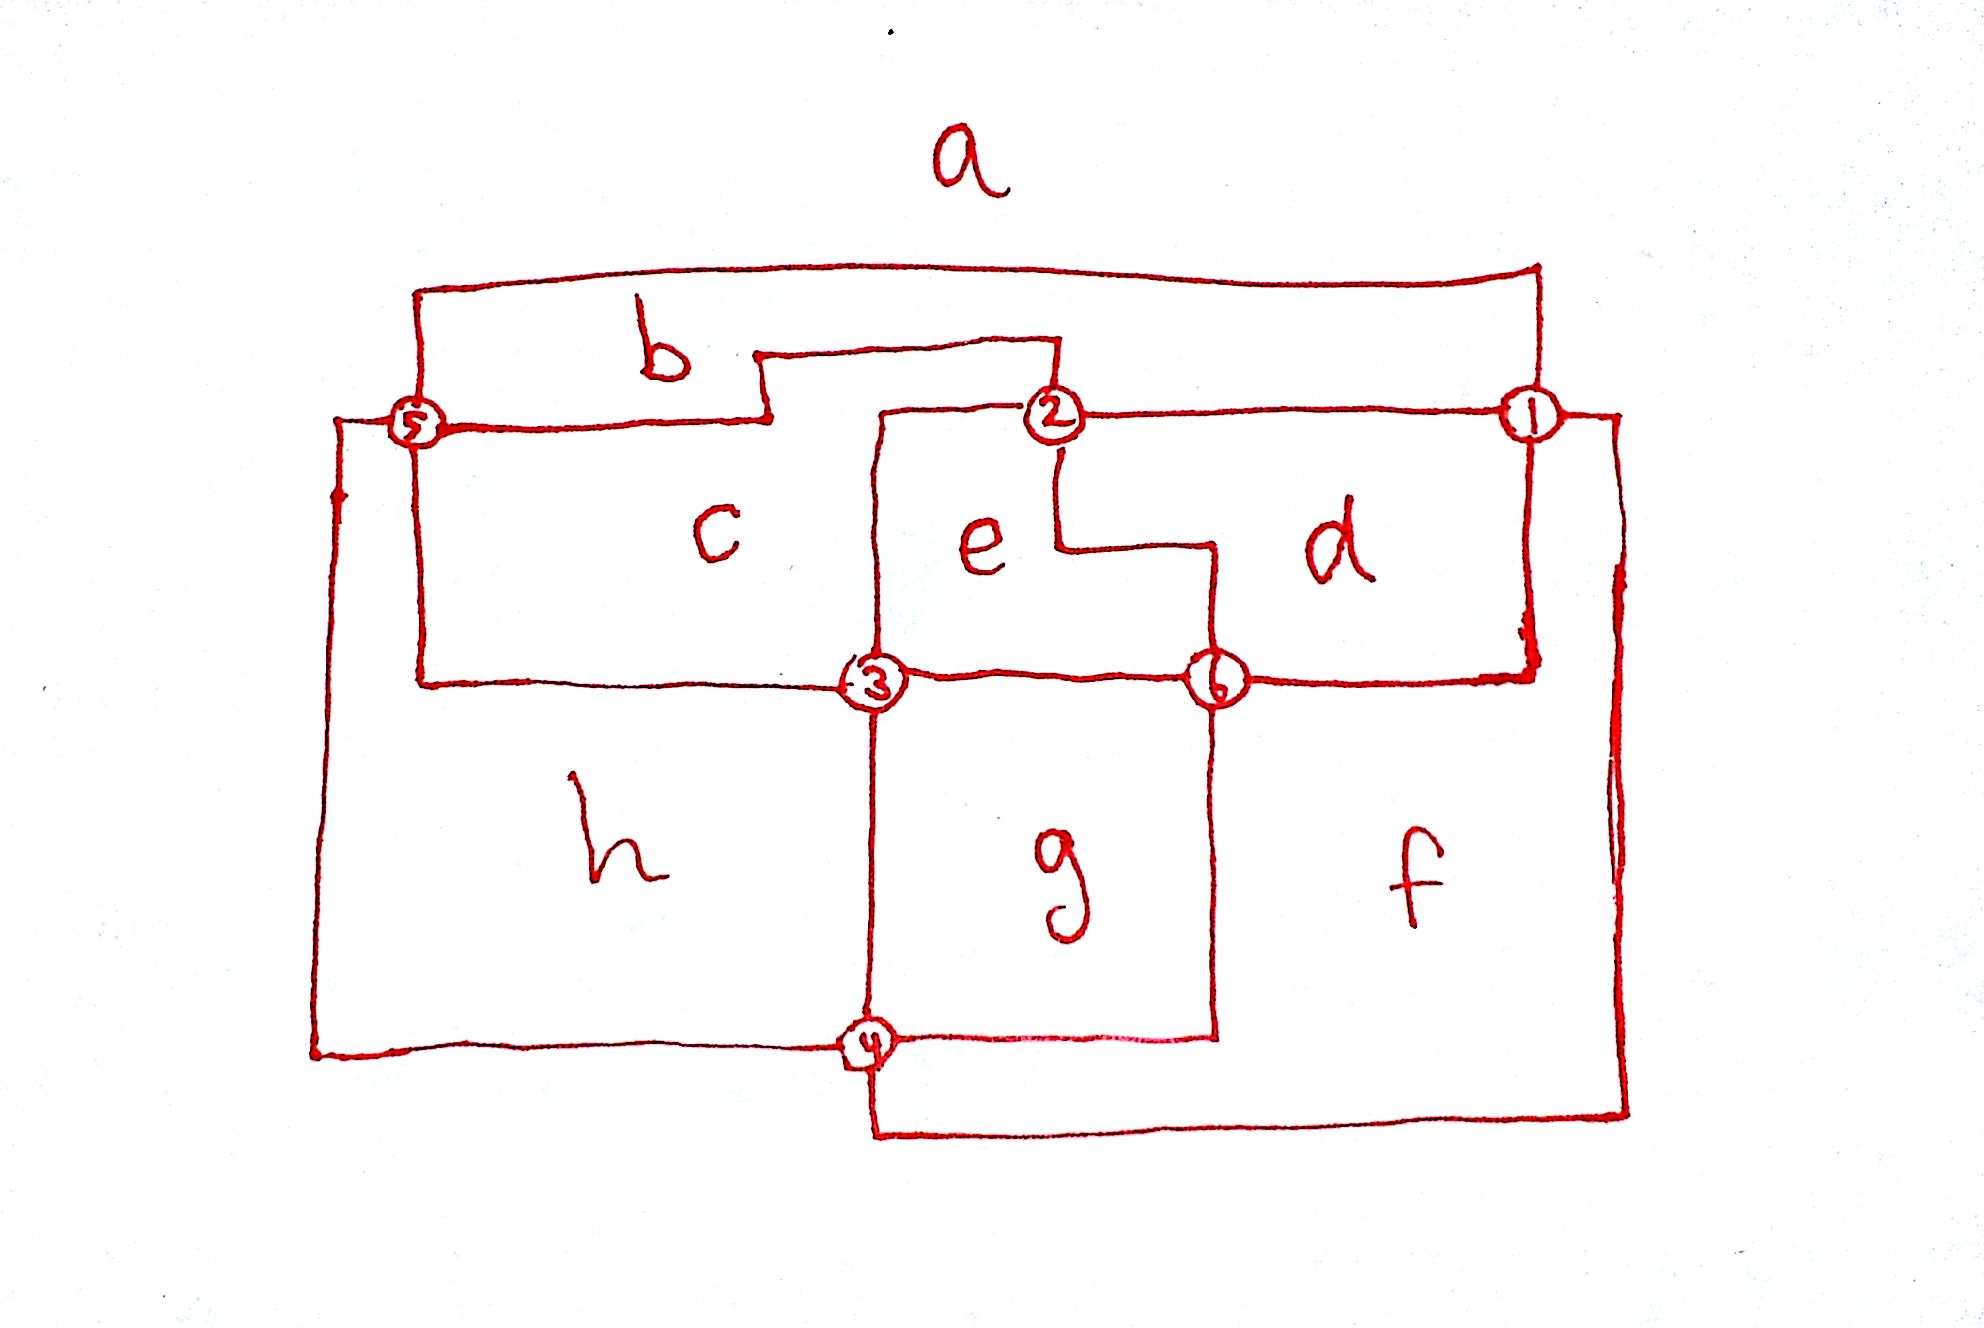
\includegraphics[width=0.5\textwidth]{images/rectilinear-2}

\subsection{3.2}
The constraints can be expressed as:

\begin{align*}
    \forall f \in F_i: &\sum_v x_{vf} + \sum_g (z_{fg} - z_{gf}) = 4 \\
                       &\sum_v x_{vf_e} + \sum_g (z_{f_eg} - z_{gf_e}) = -4
\end{align*}

\noindent where $F_i$ is the set of internal faces, and $f_e$ is the external face. 

Since we have all values for $z_{fg}$ and $x_{vf}$, verification for the boundary cycles
$a$ and $e$ is easy:

\begin{align*}
    \sum_v x_{vf_a} + \sum_g (z_{ag} - z_{ga}) &= 3 + (-7) \\
                                               &= -4 \\
    \sum_v x_{vf_e} + \sum_g (z_{eg} - z_{ge}) &= (3-1) + (4-2) \\
                                               &= 4
\end{align*}

\subsection{3.3}
If any vertex has a degree higher than 4, it isn't possible to make a
rectilinear embedding. The constraint of all edges having to be horizontal or
vertical leaves only 4 possible places for the edge to exit a vertex (top,
bottom, left, right).

We now wish to prove, that

\[
    \sum_f x_{vf} = \begin{cases} 0 & \text{if $v$ has degree $2$} \\
                                      2 & \text{if $v$ has degree $3$} \\
                                      4 & \text{if $v$ has degree $4$.} \end{cases}
\]

If $v$ has degree $2$, we have two cases:

\begin{itemize}
    \item If the edges enter the vertex opposite each other, none of the
          adjacent faces have any inner turns in the vertex, making the sum $0$.
    \item Otherwise, there will be two faces adjacent to the vertex, one of
          which has an inner turn, the other having an outer turn. This gives us a
          sum of $1 + (-1) = 0$.
\end{itemize}

If $v$ has degree $3$, we have only one case: One adjacent face\footnote{The
one facing the site without an edge.} has no inner turns, while there are two
adjacent faces containing an inner turn. This yields a sum of $0+1+1 = 2$.

If $v$ has degree $4$, we again have only one case: Four adjacent faces, each
have an inner turn. This leaves us with the sum $1+1+1+1=4$.

\subsection{3.4}
Since each break point is an inner turn for precisely one face, the sum

\[
    \sum_f \sum_g z_{fg}
\]

yields the total number of break points in the entire graph. Minimizing this
sum will therefore minimize the number of break points.

This gives us the following linear program:

\begin{align*}
    minimize & \sum_f \sum_g z_{fg} \\
    s.t.     & \\
             % constaints from 3.2 
             & \forall f \in F_i: \sum_v x_{vf} + \sum_g (z_{fg} - z_{gf}) = 4 \\
             & \sum_v x_{vf_e} + \sum_g (z_{f_eg} - z_{gf_e}) = -4 \\
             % constaints from 3.3 
             & \forall v \in V_2: \sum_f x_{vf} = 0 \\
             & \forall v \in V_3: \sum_f x_{vf} = 2 \\
             & \forall v \in V_4: \sum_f x_{vf} = 4 \\
             % non-negativity
             & \forall f, g: z_{fg} \geq 0 
\end{align*}

where $V_n$ is the set of vertices of degree $n$.

\subsection{3.5}
% TODO

\bibliographystyle{plain}
\bibliography{references.bib}
\end{document}
